\documentclass[a4paper,11pt,twoside]{article}
% Encoding lokal, da manche Editoren danach schauen
\usepackage[utf8]{inputenc} 
\usepackage{ihr-15}

\title{Benutzerhandbuch „Interaktiver Haushaltsrechner“}
 
\date{Version vom 1. Oktober 2015}

\begin{document}
\maketitle
\tableofcontents
\newpage
\seitezwei
\newpage

\section{Einleitung}
Das vorliegende Benutzerhandbuch soll Ihnen eine leichte Einf\"uhrung in
Aussehen und Bedienung unserer Website vermitteln. Alle M\"oglichkeiten werden
mit Hilfe von Bildern beschrieben.
\section{Registrieren und Anmelden}
\subsection{Registrierung}
Um die erweiterten Funktionen des interaktiven Haushaltsrechners nutzen zu
können, müssen Sie ein registrierter Benutzer sein. Dazu befindet sich auf
jeder Seite in der oberen rechten Ecke ein Registrieren- und ein Login-Link,
welche Sie zu den jeweiligen Seiten f\"uhren.
\begin{figure}[ht]
  \begin{center}
    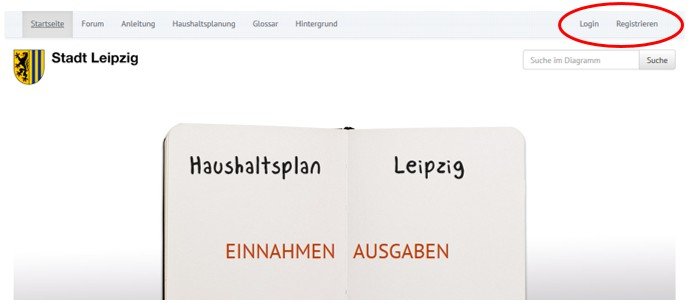
\includegraphics[width=.8\textwidth]{Bilder/anmeldung.jpg}
  \end{center}
  \caption{Einstiegsseite}
\end{figure}

Nachdem Sie auf Registrieren gedr\"uckt haben, kommen Sie auf die
Registrierungsseite, auf der Sie sich nach Eingabe der mit einem * markierten
Informationen durch einen Klick auf „Neues Benutzerkonto erstellen“ ein
Benutzerkonto f\"ur den Haushaltsrechner Leipzig erstellen können.
\begin{figure}[ht]
\begin{center}
  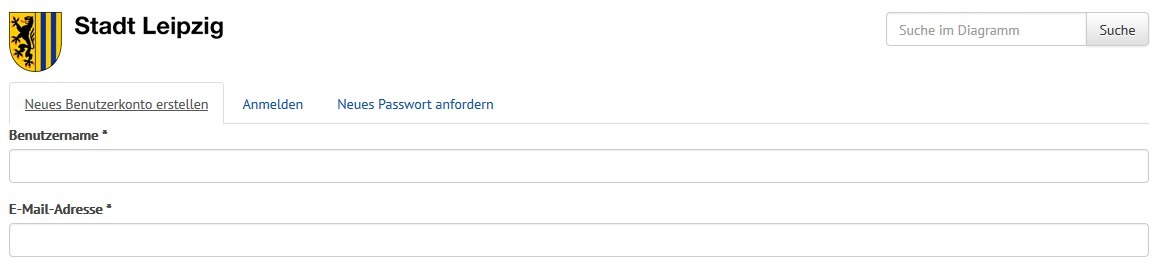
\includegraphics[width=.8\textwidth]{Bilder/registrierung.jpg}
\end{center}
  \caption{Registrierung}
\end{figure}

\subsection{Anmeldung} \label{anmeldung}
Sofern Sie schon ein Konto besitzen und sich nur anmelden wollen, um das Forum
und die Vorschlagsfunktion nutzen zu k\"onnen, m\"ussen Sie auf Login
dr\"ucken.  Nach der Eingabe Ihres Benutzernamens und Passworts dr\"ucken Sie
auf „Anmelden“.
\begin{figure}[ht]
\begin{center}
  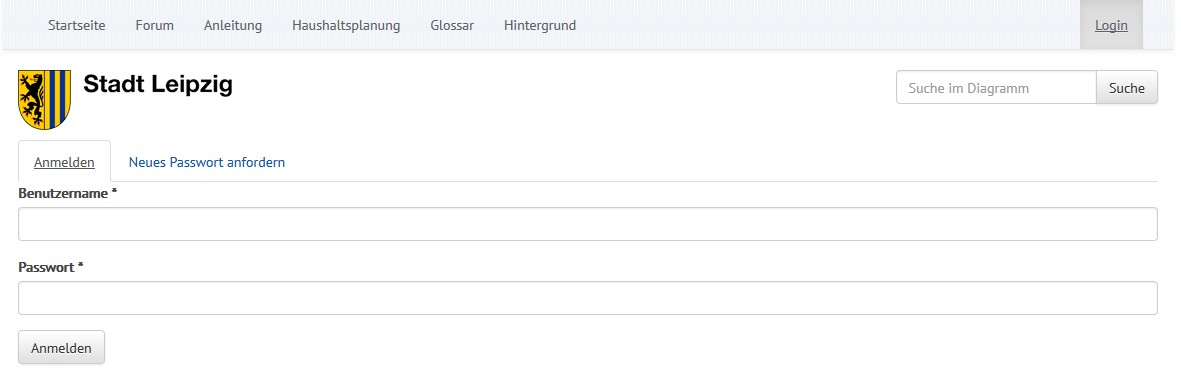
\includegraphics[width=.8\textwidth]{Bilder/anmelden.jpg}
\end{center}
  \caption{Anmeldung}
\end{figure}

\subsection{Passwort vergessen}
Sofern Sie ihr Passwort vergessen haben, k\"onnen Sie dieses durch Angabe
ihres Benutzernamens oder ihrer Email zur\"ucksetzen. Sie bekommen dann in
einer Email ein neues Passwort zugeschickt. Diese Seite ist erreichbar, indem
Sie entweder von der Registrierungsseite oder der Loginseite auf „Neues
Passwort anfordern“ dr\"ucken.
\begin{figure}[ht]
\begin{center}
  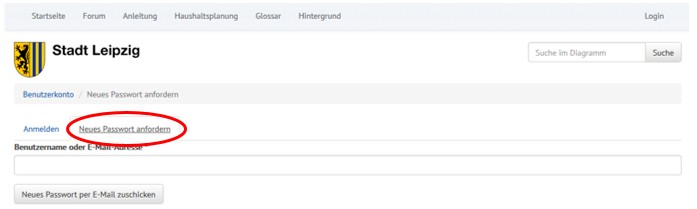
\includegraphics[width=.8\textwidth]{Bilder/neuesPasswort.jpg}
\end{center}
  \caption{Neues Passwort}
\end{figure}
\section{Haushaltsplan}

\begin{figure}[ht]
  \begin{center}
    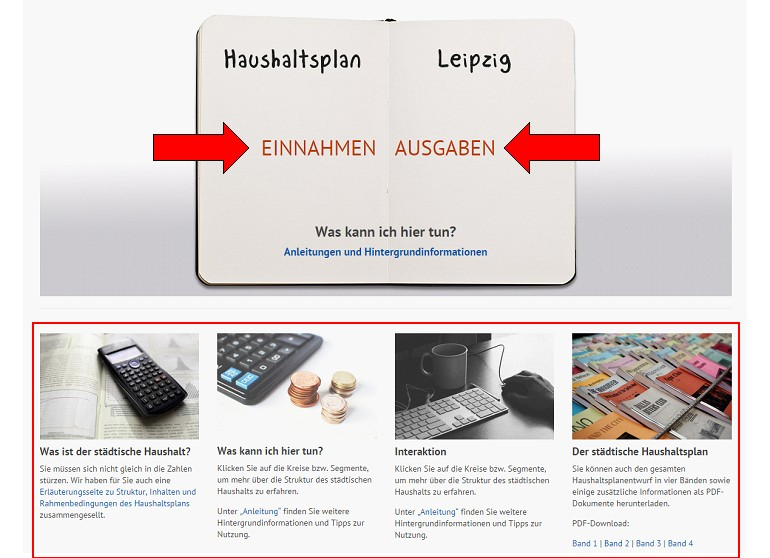
\includegraphics[width=.8\textwidth]{Bilder/einAus.jpg}
  \end{center}
  \caption{Einstiegsseite des Haushaltsrechners}
\end{figure}

Auf der Startseite des Interaktiven Haushaltsplans (auf diese gelangen Sie von
jeder anderen Seite, indem Sie auf das Logo der Stadt Leipzig oder auf den
Link „Startseite“ in der oberen Menüleiste klicken) sehen Sie das
Haushaltsbuch der Stadt Leipzig. Per Klick k\"onnen Sie sich hier zwischen der
Ansicht auf die Einnahmen oder die Ausgaben der Stadt entscheiden.

Daneben finden Sie unter dem Haushaltsbuch Links zu weiterführenden
Informationen über den städtischen Haushalt, eine Kurzanleitung, wie der
Haushaltsrechner funktioniert und Verweise auf die PDF-Dateien des städtischen
Haushalts.
\enlargethispage{2em}

\subsection{Einnahmen \& Ausgaben}
\begin{figure}[ht]
\begin{center}
  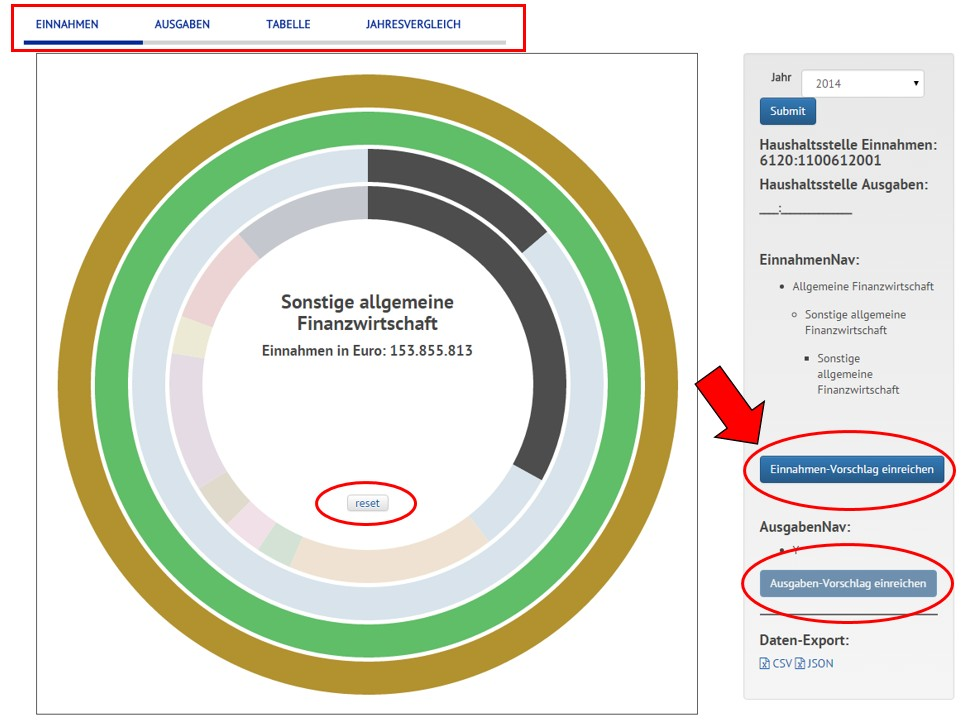
\includegraphics[width=\textwidth]{Bilder/piechart.jpg}
\end{center}
  \caption{Vorschlag einreichen}
\end{figure}

Nach einem Klick auf „Einnahmen“ bzw. „Ausgaben“ gelangen Sie in das Herzstück
des Interaktiven Haushaltsrechners. Hier sehen Sie ein Kreisdiagramm, welches
prozentual die Einnahmen bzw. Ausgaben für die verschiedenen Haushaltsposten
der Stadt Leipzig anzeigt.
 
Sobald Sie im Diagramm auf ein eingefärbtes Segment des Kreises klicken,
öffnen sich die zu diesem Haushaltsposten gehörigen Unterposten. In diesem neu
geöffneten Kreis, der die Unterposten anzeigt, können Sie sich durch Klick auf
ein Segment wiederum die jeweiligen zugehörigen Haushaltsposten anzeigen
lassen -- insgesamt gibt es so bis zu drei weitere Ebenen, also vier Kreise.
Wenn Sie neu mit dem Klicken durch das Diagramm beginnen wollen, können Sie
jederzeit auf den Button „Reset“ in der Mitte des Kreises klicken.

Wenn Sie mit der Maus \"uber einen Bereich im Kreisdiagramm gehen, sehen Sie
in der Mitte des Diagramms den Namen des Haushaltspostens sowie dessen
zugehörigen Geldbetrag. Zu beachten ist, dass in jedem Kreis auch ein Segment
mit dem Namen „Sonstiges“ vorhanden ist, welches nicht klickbar ist, sondern
eine Zusammenfassung aller Bereiche, welche weniger als 2\,\% der Einnahmen
bzw. Ausgaben ausmachen, darstellt. Diese sind im Tab „Tabelle“ genauer
aufgelistet und klickbar.

Über das Menü direkt über dem Kreisdiagramm können Sie jederzeit zwischen den
Ansichten „Einnahmen“, „Ausgaben“, „Übersichtstabelle“ und „Jahresvergleich“
wechseln. Rechts vom Kreisdiagramm sehen Sie einen Block, in dem die
Informationen zu den Haushaltsposten, die Sie in den Diagrammen bzw. der
Tabelle angeklickt haben, zusammengefasst angezeigt werden.  Beachten Sie
dabei auch, dass die Navigation durch die Einnahmen und Ausgaben getrennt
voneinander funktioniert: Wenn sie z.B. bei den Einnahmen ein Kreissegment
anklicken, ändert sich beim Kreisdiagramm der Ausgaben nichts.
\enlargethispage{2em}

\subsubsection{Vorschlag einreichen}
Sobald Sie auf einen Haushaltsposten geklickt haben können Sie -- sofern Sie
bereits als Benutzer angemeldet sind (siehe Punkt \ref{anmeldung}) -- im
Infoblock rechts neben dem Kreisdiagramm bzw. der Tabelle auf den Button
„Einnahmen-Vorschlag einreichen“ bzw. „Ausgaben-Vorschlag einreichen“
klicken. Sie werden dann zum Forum weitergeleitet, wo Sie Ihren Vorschlag zur
Verbesserung des städtischen Haushalts öffentlich niederschreiben können
(siehe Punkt \ref{vorschlag}).

\subsection{Tabelle}
Nach einem Klick auf den Reiter „Tabelle“ im Schnellmenü über dem
Kreisdiagramm erscheint eine Tabelle, welche genauere Angaben zu den in den
Einnahmen- und Ausgaben-Kreisdiagramm gedr\"uckten Bereichen enth\"alt. Die
Tabelle ist genauso wie die Kreisdiagramme klickbar.

\subsection{Jahresvergleich}
Unter dem Reiter „Jahresvergleich“ erscheinen für das zuletzt ausgewählte
Kreissegment die zugehörigen Einnahmen und Ausgaben in tabellarischer Form
verglichen mit anderen Haushaltsjahren.

\section{Forum}
Im Forum k\"onnen f\"ur die einzelnen Produktbereiche des Haushaltsplans
Vorschl\"age gelesen, bewertet, kommentiert und erstellt werden. Weiterhin
gibt es die Foren „Allgemeine Diskussion“ und „Offizielle Diskussion“, in
denen übergreifende Probleme diskutiert werden können. Um im Forum zu lesen,
ist keine Anmeldung notwendig, f\"ur alle im Weiteren genannten Funktionen ist
sie eine Anmeldung erforderlich.

\begin{figure}[ht]
\begin{center}
  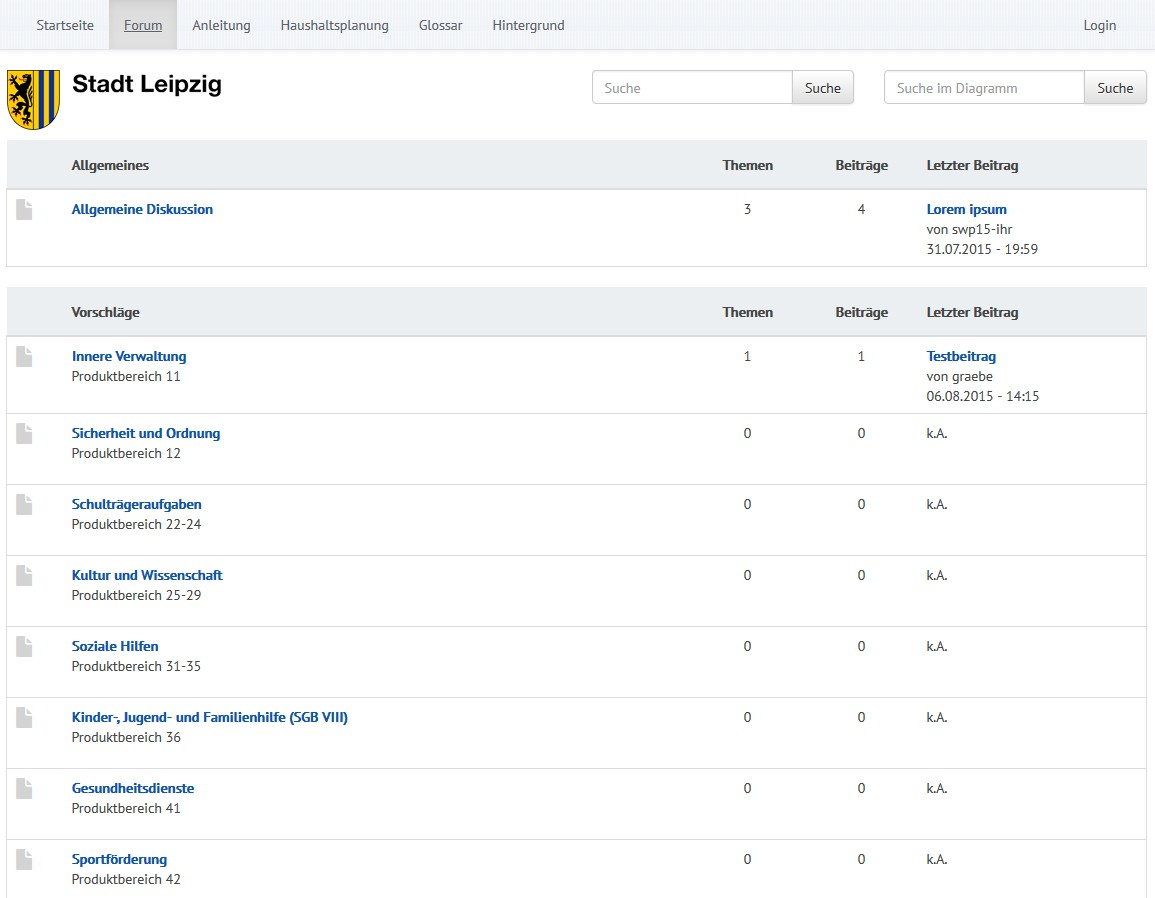
\includegraphics[width=\textwidth]{Bilder/forum.jpg}
\end{center}
  \caption{Forumsbereich des Haushaltsrechners}
\end{figure}

\subsection{Vorschlag erstellen} \label{vorschlag}
Einen neuen Vorschlag erstellen Sie, indem Sie auf ein Forum des jeweiligen
Produktbereichs klicken (in diesem Beispiel „Kultur und Wissenschaft“) und auf
Forenthema hinzuf\"ugen dr\"ucken.

\begin{figure}[ht]
\begin{center}
  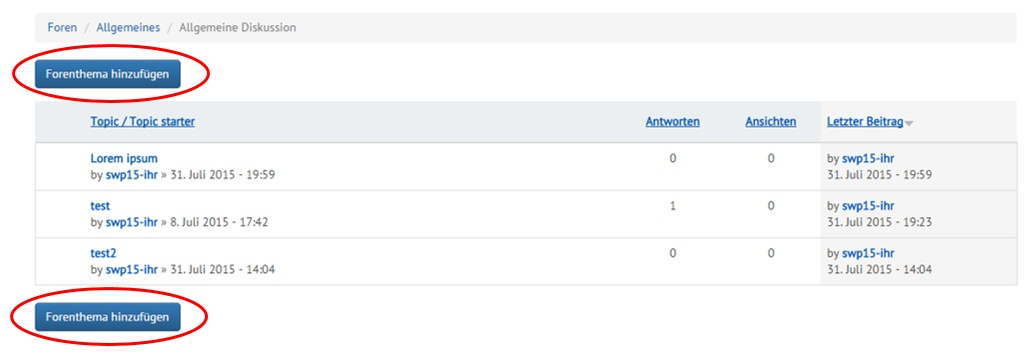
\includegraphics[width=\textwidth]{Bilder/forumtopic.jpg}
\end{center}
  \caption{Vorschlag erstellen}
\end{figure}

\subsection{Vorschl\"age sortieren und anschauen}
Sofern Sie auf einen Bereich gedr\"uckt haben, sehen Sie alle Vorschl\"age in
diesem Bereich jeweils mit Titel, Autor, Datum, Antworten, Anzahl der
Personen, die sich diesen Vorschlag angeschaut haben, und Autor des letzten
Kommentares.

Wenn Sie auf die Überschriften klicken, k\"onnen Sie die Beitr\"age nach
gewissen Eigenschaften sortieren. Um die Sortierrichtung zwischen auf- und
absteigend zu wechseln, müssen Sie erneut auf die jeweilige Überschrift
klicken.

\begin{figure}[ht]
\begin{center}
  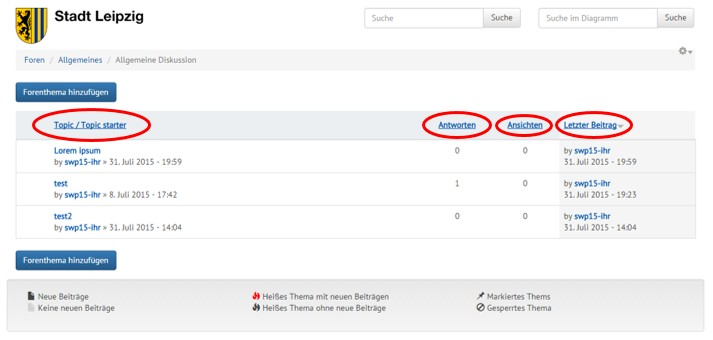
\includegraphics[width=\textwidth]{Bilder/forumsort.jpg}
\end{center}
  \caption{Beiträge sortieren}
\end{figure}

\subsection{Vorschl\"age kommentieren, bewerten und melden}
Nachdem Sie auf einen Vorschlag geklickt haben, gelangen Sie auf dessen
Detailseite, wo Sie den entsprechenden Text lesen können.

Um einen Kommentar zu erstellen, schreiben Sie einfach ihren gewünschten Text
in die daf\"ur vorgesehene Textbox und dr\"ucken auf „Vorschau“, um zu sehen,
wie Ihre Nachricht aussehen w\"urde. Anschließend können Sie auf „Speichern“
klicken, damit Ihr Kommentar zum Vorschlag im Forum abgelegt wird.

Unter dem Text des Vorschlags-Autors k\"onnen Sie außerdem durch Dr\"ucken von
$+$ oder $-$ eine Bewertung des Vorschlags zum städtischen Haushalt abgeben.
Wenn Sie sich später wieder anders entscheiden, kann diese wieder durch
Dr\"ucken des anderen Buttons ge\"andert werden.

Falls aus Ihrer Sicht ein Beitrag gegen die Nutzungsbedingungen des
Interaktiven Haushaltsrechners verstößt, können Sie diesen per Klick auf den
roten „Missbrauch melden“-Button an die Redaktion melden, welche sich so
schnell wie möglich um eine Prüfung kümmern wird.

\subsection{Bürgereinwand einreichen}

Ein wichtiges Instrument zur Bürgerbeteiligung ist der Bürgereinwand.  Diese
Funktion steht nur während der offiziellen Auslage des Haushaltsentwurfs zur
Verfügung und erlaubt es Ihnen, per Klick auf den hellblauen
„Bürgereinwand“-Button aus dem Vorschlagsthema einen digitalen Bürgereinwand
an die Stadt Leipzig zu machen, der unter Ihrem Namen in die
Haushaltsdiskussion eingebracht wird und den gleichen rechtlichen Status wie
alle anderen schriftlich eingereichten Bürgereinwände hat.

Das nähere Verfahren des Umgangs mit solchen digitalen Bürgereinwänden ist in
der Stadtverwaltung noch im Klärungsprozess.

\begin{figure}[ht]
\begin{center}
  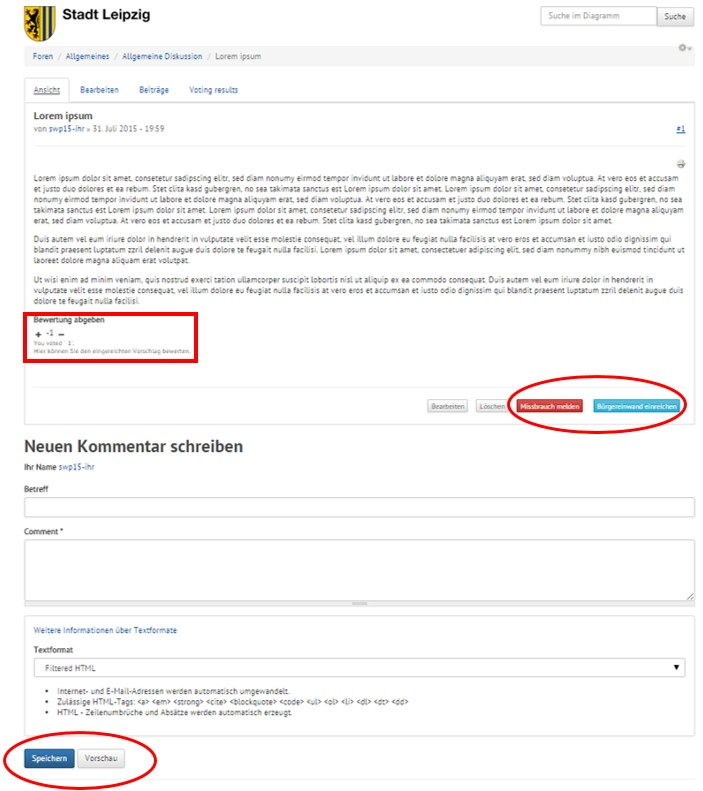
\includegraphics[width=\textwidth]{Bilder/comment.jpg}
\end{center}
  \caption{Weitere Kommentarfunktionen}
\end{figure}
\end{document}
